\documentclass[12pt]{article}
\usepackage{graphicx}
\usepackage{amsmath}
\usepackage{amssymb}
\usepackage{amstext}
\usepackage{amsfonts}
\usepackage{mathrsfs}
\usepackage{makeidx}
\usepackage{multirow}
\usepackage{pgfplots }
\setlength{\parindent}{0pt}
\title{STEM Gender Gap in University Education}
\date{June 2017}
\author{Peter Pointner ,Thomas Sulzbacher, Yang Hua}

\begin{document}
	\pagenumbering{gobble}
	\maketitle
	\newpage
	
	\tableofcontents
	\newpage
	\pagenumbering{arabic}
	\section{Abstract}
In this paper our team focuses on the gender gap which appears in Science Technology Engineering Mathematics and Computer ,henceforth STEM, majors in university education. First of all we want to give an overview of the current situation of inscription rates in different STEM related majors at Johannes Kepler University Linz, from now on  JKU, and how the development progressed from 2002 to 2016 based on \cite{studienwahl_jku} \cite{eq_1} \cite{eq_2} \cite{eq_3}. After taking a close look at the situation in Austria we want to focus on reasons for the decision made when choosing a university major and what different influences people are committed.
In the next section the gender gap in STEM majors on universities in Germany is evaluated and compared against the situation in Austria. The main focus ,of the second part of this report, is to take a closer look at the international situation of the STEM gender gap. At the end of the report a conclusion of our findings will be presented.    
 	\section{Situation in German speaking countries}
	\subsection{Situation at JKU}
The study conducted in  \cite{eq_1}\cite{eq_2}\cite{eq_3}  showed that from 2005 throughout 2016 the share between man and women studying at JKU was not reflecting the demographic composition of Austria which would be 51\% women and 49\% of men studying at JKU. In 2005  the share between man and women studying at JKU was at a rate of  45\% but there is a slight increase since 2005 to 2016 where 49\% of all students at JKU were female students. If a closer look is taken at the inscription rates of new students, the rate of women starting at JKU in 2016, we see that the share of women is 53\%, which also represents the mean of female students of all Austrian universities. From the gender equality reports conducted from 2005 to 2016 it can be seen that JKU has a general problem in attracting women but the problem minimized during the past years. \newline\newline
After describing the general share of female and male students at JKU a closer look is now taken at the STEM related majors.
Unfortunately the data presented in \cite{eq_1}\cite{eq_2}\cite{eq_3} is inconsistent with each other meaning some data given in \cite{eq_1}can not be found in \cite{eq_2} and \cite{eq_3} or is structured in a different way. First we want to take a look at the statistics for the whole Technical faculty of Natural Science, hence TNF.\newline
\begin{figure}[h!]
\centering
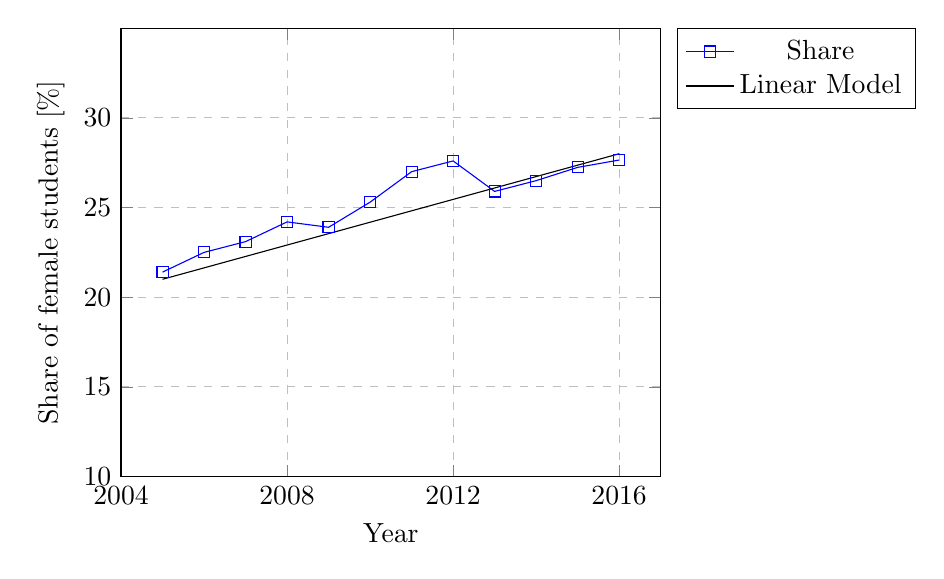
\begin{tikzpicture}
\begin{axis}[
    %title={STEM Gender Gap developement at JKU's TNF},
    	x tick label style={/pgf/number format/1000 sep=},
	xlabel={Year},
    	ylabel={Share of female students [\%]},
    	xmin=2004, xmax=2017,
    	ymin=10, ymax=35,
    	xtick={2004,2008,2012,2016},
    	ytick={0,10,15,20,25,30},
    	ymajorgrids=true,
	xmajorgrids=true,
    	grid style=dashed,
legend pos = outer north east,
]
\addplot[color=blue,mark=square,]
    coordinates {(2005,21.4)(2006,22.5)(2007,23.1)(2008,24.2)(2009,23.9)(2010,25.3)(2011,27.0)(2012,27.6)(2013,25.9)(2014,26.5)(2015,27.24)(2016,27.65)};
\addplot[color=black,mark=point,]
    coordinates {(2005,21)(2016,28)};
\legend{Share,Linear Model}
\end{axis}
\end{tikzpicture}
\caption[Developement of STEM Gap at JKU]{STEM Gender Gap developement at JKU's TNF.}
\label{fig:dev}
\end{figure}
\subsection{Situation in Germany}
In figure number \ref{fig:dev} we can see the development of the STEM Gap at JKU's TNF over a periode of 11 Years. If   a linear regression model is assigned to the data ,given by the equality reports, with 
\begin{equation}
y= \frac{7}{11}*x+21.4
\end{equation}  we see that the slight increase of female students at JKU fits the chosen model pretty well and this model might be useful for further estimates of the general decrease of the STEM Gap.
If we take a closer look on the different STEM topics we notice that the STEM Gap is not found in all majors. In general it can be said that the share of male and female students in majors having a bio-science background   is dominated by female students. The share is about 63\% and keeps steady over the years. 
The highest gap which can be found at JKU is in Computer Science with only a share of 13\% female students. If the data of the equality reports is analyzed in further detail it can be seen that there is also no increase of female students in Computer Science since 2005. 

%\begin{figure}[h!]
%	\includegraphics[width=\linewidth]{vq_priciple.jpg}
%	\caption[Vector Quantization Principle Taken from: \cite{vq_2}]{Vector Quantization Principle.}
%	\label{fig:vq}
%\end{figure}
\newpage
\bibliography{gender}
\bibliographystyle{unsrt}
\newpage
\listoffigures
\listoftables
\end{document}